\chapter{Large language models}


\begin{description}
    \item[Conditional generation] \marginnote{Conditional generation}
        Generate text conditioned on the input tokens (i.e., prompt).

        \begin{figure}[H]
            \centering
            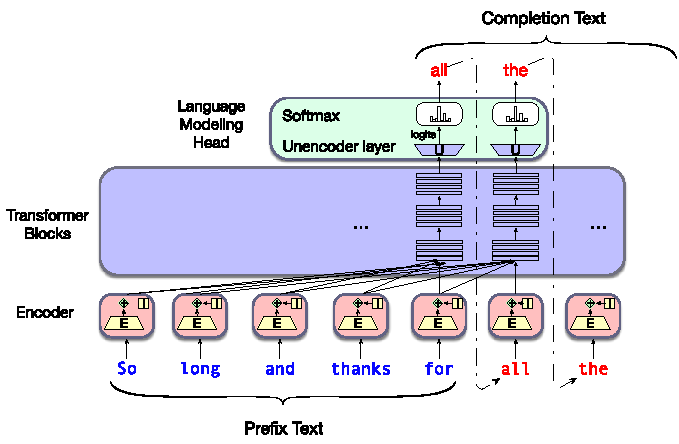
\includegraphics[width=0.45\linewidth]{./img/_conditional_generation.pdf}
        \end{figure}

        \begin{example}[Sentiment analysis]
            Given the prompt:
            \[ p = \texttt{the sentiment of the sentence `I like Jackie Chan' is} \]
            Determine the probability of the tokens \texttt{positive} and \texttt{negative}:
            \[
                \prob{\texttt{positive} \mid p} \qquad \prob{\texttt{negative} \mid p}
            \]
        \end{example}

        \begin{example}[Question answering]
            Given the prompt:
            \[ p = \texttt{Q: who wrote the book `The origin of Species'? A:} \]
            Determine the tokens of the answer autoregressively:
            \[
                \arg\max_{w_1} \prob{w_1 \mid p}, \arg\max_{w_2} \prob{w_2 \mid pw_1}, \dots
            \]
        \end{example}
\end{description}


\section{Decoding strategies}

\begin{description}
    \item[Greedy decoding] \marginnote{Greedy decoding}
        Select the next token as the most probable of the output distribution.

        \begin{remark}
            Greedy decoding risks getting stuck in a local optimum.

            \indenttbox
            \begin{example}
                Consider the following search tree of possible generated sequences:
                \begin{figure}[H]
                    \centering
                    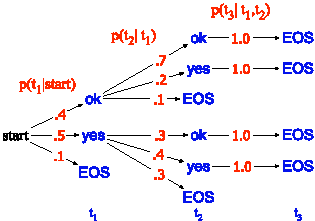
\includegraphics[width=0.3\linewidth]{./img/_greedy_decoding_local_minimum.pdf}
                \end{figure}

                Greedy search would select the sequence \texttt{yes yes} which has probability $0.5 \cdot 0.4 = 0.2$. However, the sequence \texttt{ok ok} has a higher probability of $0.4 \cdot 0.7 = 0.28$.
            \end{example}
        \end{remark}

    \item[Beam search] \marginnote{Beam search}
        Given a beam width $k$, perform a breadth-first search keeping at each branching level the top-$k$ tokens based on the probability of that sequence:
        \[ \log\left( \prob{y \mid x} \right) = \sum_{i=1}^{t} \log\left( \prob{ y_i \mid x, y_1, \dots, y_{i-1} } \right) \]

        \begin{example}
            Consider the following tree with beam width $k=2$:
            \begin{figure}[H]
                \centering
                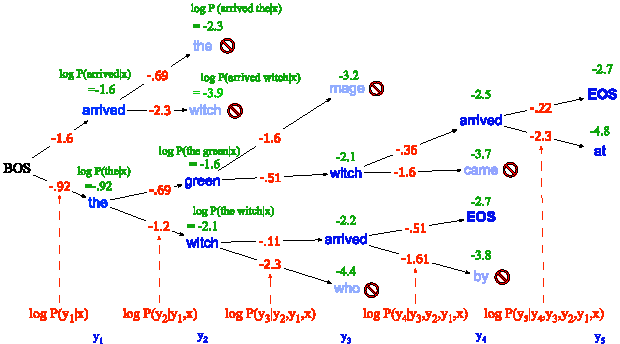
\includegraphics[width=0.7\linewidth]{./img/_beam_search.pdf}
            \end{figure}
            The selected sequence is \texttt{[BOS] the green witch arrived [EOS]}.
        \end{example}

        \begin{remark}
            As each path might generate sequences of different length, the score is usually normalized by the number of tokens as:
            \[ \log\left( \prob{y \mid x} \right) = \frac{1}{t} \sum_{i=1}^{t} \log\left( \prob{ y_i \mid x, y_1, \dots, y_{i-1} } \right) \]
        \end{remark}

        \begin{remark}
            The likelihood of the sequences generated using beam search is higher than using greedy decoding. However, beam search is still not optimal.
        \end{remark}

    \item[Sampling] \marginnote{Sampling}
        Sample the next token based on the output distribution.

        \begin{description}
            \item[Random sampling]
                Sample considering the distribution over the whole vocabulary.

                \begin{remark}
                    By adding-up all the low-probability words (which are most likely unreasonable as the next token), their actual chance of getting selected is relatively high.
                \end{remark}

            \item[Temperature sampling]
                Skew the distribution to emphasize the most likely words and decrease the probability of less likely words. Given the logits $\vec{u}$ and the temperature $\tau$, the output distribution $\vec{y}$ is determined as:
                \[ \vec{y} = \texttt{softmax}\left( \frac{\vec{u}}{\tau} \right) \]
                where:
                \begin{itemize}
                    \item Higher temperatures (i.e., $\tau > 1$) allow for considering low-probability words.
                    \item Lower temperatures (i.e., $\tau \in (0, 1]$) focus on high-probability words.
                    \begin{remark}
                        A temperature of $\tau = 0$ corresponds to greedy decoding.
                    \end{remark}
                \end{itemize}


            \item[Top-k sampling]
                Consider the top-$k$ most probable words and apply random sampling on their normalized distribution.

                \begin{remark}
                    $k=1$ corresponds to greedy decoding.
                \end{remark}

                \begin{remark}
                    $k$ is fixed and does not account for the shape of the distribution.
                \end{remark}

            \item[Top-p/nucleus sampling]
                Consider the most likely words such that their probability mass adds up to $p$. Then, apply random sampling on their normalized distribution.
        \end{description}
\end{description}



\section{Training}


\subsection{Pre-training}

\begin{description}
    \item[Pre-training] \marginnote{Pre-training}
        Use self-supervision and teacher forcing to train the whole context window in parallel on a large text corpus.

        \begin{remark}
            Results are highly dependent on the training corpora. Important aspects to consider are:
            \begin{descriptionlist}
                \item[Language] Most of the available data is in English.
                \item[Data quality] Prefer high-quality sources such as Wikipedia or books. Boilerplate removal and deduplication might be needed. 
                \item[Safety filtering] Toxicity removal might be needed
                \item[Ethical and legal issues] Use of copyrighted material, permission from data owners, use of private information, \dots
            \end{descriptionlist}
        \end{remark}

    \item[Scaling laws] \marginnote{Scaling laws}
        Empirical laws that put in relationship:
        \begin{itemize}
            \item Non-embedding parameters $N$ ($N \approx 2 d_\text{model} n_\text{layer} (2 d_\text{attention} + d_\text{ff})$),
            \item Training data size $D$,
            \item Compute budget $C$ (i.e., training iterations).
        \end{itemize}
        By keeping two of the three factors constant, the loss $\mathcal{L}$ of an LLM can be estimated as a function of the third variable:
        \[ 
            \mathcal{L}(N) = \left( \frac{N_c}{N} \right)^{\alpha_N} 
            \qquad
            \mathcal{L}(D) = \left( \frac{D_c}{D} \right)^{\alpha_D} 
            \qquad
            \mathcal{L}(C) = \left( \frac{C_c}{C} \right)^{\alpha_C} 
        \]
        where $N_c$, $D_c$, $C_c$, $\alpha_N$, $\alpha_D$, and $\alpha_C$ are constants determined empirically based on the model architecture.
\end{description}


\subsection{Fine-tuning}

\begin{description}
    \item[Fine-tuning] \marginnote{Fine-tuning}
        Specialize an LLM to a specific domain or task.

        \begin{description}
            \item[Continued pre-training] \marginnote{Continued pre-training}
                Continue pre-training with a domain-specific corpus.

            \item[Model adaptation]
                Specialize a model by adding new learnable parameters.

                \begin{description}
                    \item[Parameter-efficient fine-tuning (PEFT)] \marginnote{Parameter-efficient fine-tuning (PEFT)}
                        Continue training a selected subset of parameters.

                        \begin{description}
                            \item[Low-rank adaptation (LoRA)] \marginnote{Low-rank adaptation (LoRA)}
                                Method to update weights by learning an offset that uses fewer parameters.

                                Consider a weight matrix $\matr{W} \in \mathbb{R}^{d \times k}$, LoRA decomposes the update into two learnable matrices $\matr{A} \in \mathbb{R}^{d \times r}$ and $\matr{B} \in \mathbb{R}^{r \times k}$ (with $r \ll d, k$). Weights update is performed as:
                                \[ \matr{W}_{\text{fine-tuned}} = \matr{W}_{\text{pre-trained}} + \matr{AB} \]

                                \begin{figure}[H]
                                    \centering
                                    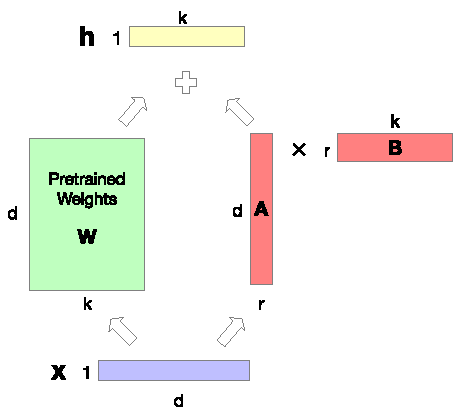
\includegraphics[width=0.35\linewidth]{./img/_lora.pdf}
                                \end{figure}
                        \end{description}

                    \item[Task-specific fine-tuning] \marginnote{Task-specific fine-tuning}
                        Add a new trainable head on top of the model.
                \end{description}

            \item[Supervised fine-tuning] \marginnote{Supervised fine-tuning}
                Continue training using a supervised dataset to align the model to human's expectation.
        \end{description}
\end{description}